\documentclass[11pt,a4paper]{article}
\usepackage{fontspec}
\usepackage[english]{babel}
\usepackage[margin=2.1cm]{geometry}
\usepackage{booktabs,array,tabularx}
\usepackage{xcolor}
\usepackage{graphicx}
\usepackage{pgfplots}
\pgfplotsset{compat=1.17}
\PassOptionsToPackage{hyphens}{url}
\usepackage[hidelinks]{hyperref}
\usepackage{enumitem}
\setlist{nosep,leftmargin=1.4em}
\emergencystretch=3em

\definecolor{impl}{HTML}{3B6EA8}
\definecolor{rev}{HTML}{8FB3DA}
\definecolor{waste}{HTML}{C8553D}

\title{Sweatshop on P-Chess: Review exploration\\\large Side lines in the Review (REV-007), engine lines and live Stockfish (REV-008) and live classes for side-line moves (REV-009); GPT-6.1 Terra lineup, lane \texttt{review-explore}}
\author{Foreman, session \texttt{sweatshop/review-explore/2026-11-05-1723}}
\date{5 November 2026}

\begin{document}
\maketitle

\section*{Summary}

First run of the \texttt{review-explore} lane, in a new clone at
\path{.artifacts-build/lanes/review-explore} made from \texttt{main} at \texttt{184a0bf} (the spec
and tickets from Bruno's grilling the same day). Three launches: 17:23 (one stage, then nothing
runnable), 17:39 after the environmental fix, 18:21 after the reopen diagnosis. Last merge at 20:04,
session PR \href{https://github.com/Laginho/P-Chess/pull/42}{\#42}.

\begin{itemize}
  \item \textbf{Produced:} the lane's three tickets merged on the session with
        \texttt{Verdict: Approve}: REV-008 and REV-009 (\texttt{Review: human}: Bruno checks them
        with real Stockfish on Windows before merging into \texttt{main}) and REV-007
        (\texttt{Review: agent}). One follow-up filed by review: CLEAN-014 (needs-triage).
  \item \textbf{Cost:} \textbf{\$11.40} at API list price over 15 stages, all priced:
        \texttt{gpt-6.1-terra xhigh} implementing \$1.41 (3), \texttt{gpt-6.1-sol xhigh}
        implementing hard tickets \$4.57 (5), \texttt{gpt-6.1-sol xhigh} reviewing \$5.43 (7).
        Codex quota: 8 points of the weekly window (Sol xhigh 4: 2 implementing, 2 reviewing; Terra
        xhigh 0; 4 outside the stages, mostly the EasyMath \texttt{infra} lane running at the same
        time and one foreman \texttt{codex exec} check; $\pm$1 per stage, the total is exact), no
        reset. Plan: the account's Codex plan, shared with the EasyMath lane.
  \item \textbf{What went wrong:} the first stage never loaded \texttt{ticket-flow}: the skills were
        not installed for Codex on the Linux box (no \path{~/.agents/skills}) and P-Chess's
        \path{AGENTS.md} does not tell a bare-id prompt to load it. The stage coded REV-007 straight
        on the session, with no branch, commits or test-first, and the driver parked it. Then
        REV-007 took three reopens, the last two on narrower variants of the same Settings-access
        criterion.
  \item \textbf{Provisional verdict:} the feature is built and reviewed with real viewport input
        and fake engines. Its central risk, live Stockfish, is unexamined: no engine runs on this
        machine. Bruno's Windows check is the gate to \texttt{main}.
\end{itemize}

\section*{What was done}

\textbf{REV-007}: in the Review you can now play your own move from any position of the game (drag
or click-click). It starts one temporary side line, listed as extra rows under the branching move
with a \textbf{Back to game} button. Arrows and Previous/Next walk the line; clicking a game move,
the graph, First/Last, Back to game or Esc leaves it, and nothing of it is saved or exported. A new
\emph{Best move arrow} setting (default on) draws the stored best move in translucent blue on game
positions, and the Review's board now follows the board preferences live. Main files
\path{ui/review.gd}, \path{ui/main.gd}, \path{ui/board_view.gd}, \path{core/settings.gd}.
Reopened three times:
(1) the Review board ignored real mouse input: \path{ui/review.tscn} left it at
\texttt{MOUSE\_FILTER\_IGNORE}, and the tests called \texttt{board.play()} directly. Settings could
not open over the Review: \texttt{\_covers\_settings()} in \path{ui/main.gd} saw Review above
it. Moves lost their animation because assigning \texttt{board.game} ran the setter's
\texttt{\_end\_slide()}.
(2) Settings was still unreachable in a Review opened from a focus-mode game: \texttt{\_set\_focus}
in \path{ui/main.gd} hides it and \path{ui/game_over.gd}'s Review never restores it.
(3) after an agreed draw in focus mode, the non-modal draw notice counted as a covering screen and
blocked Ctrl+, for up to 3 seconds (\path{ui/main.gd}).

\textbf{REV-008}: a two-row \emph{engine lines} block sits between the eval graph and the move
list. Each row has an eval chip (White's view) and the line in SAN, with the depth on the first
row. Game positions show their stored lines. In a side line the Review starts its own Stockfish
(MultiPV 2, unlimited search on the shown position) and pauses the background analysis queue
until you leave the line. Clicking a move in a line plays up to it. Main files
\path{engine/live_analysis.gd} (new), \path{ui/review.gd}, \path{engine/uci.gd}. Not reopened.

\textbf{REV-009}: each side-line move gets its class icon (on the square and in its row) once both
its positions have settled: the analysis node budget, or converged depths. The same
\texttt{Classification.evaluate} as game moves computes it, and it then stays fixed. The green
``should have played'' arrow works on side-line moves too. Main files
\path{engine/live_analysis.gd}, \path{ui/review.gd}. Reopened once:
(1) a game that ended in a draw has stored terminal analysis with an empty PV. Reused as the
before-position of a legal explored move, it made \texttt{Classification.evaluate} read out of
bounds and the move stayed unclassified (\path{ui/review.gd}, \texttt{\_line\_positions}).
Returning to an already settled position also stopped the live search and showed the older frozen
lines: \texttt{\_next\_fen} in \path{engine/live_analysis.gd} returned nothing once a class
existed.

No roadmap image: P-Chess's \path{AGENTS.md} has no \texttt{Roadmap:} binding.

\section*{Timeline}

{\small
\begin{tabularx}{\linewidth}{@{}lX@{}}
\toprule
17:22 & Clone made from \texttt{184a0bf}, \texttt{godot --import}; the generated untracked
        \texttt{.uid}/\texttt{.import} files removed so Preflight sees a clean tree. \\
17:23--17:37 & Launch 1, default lineup (Terra). REV-007 stage 2 codes without \texttt{ticket-flow}:
        no branch, no commit; parked as incomplete handoff, work stashed for recovery. \\
17:38 & Foreman links the Agent-Skills skills into \path{~/.agents/skills} (the README's Codex
        path); \texttt{codex exec} lists \texttt{ticket-flow}. REV-007 back to
        \texttt{to-implement}. \\
17:39--17:49 & Launch 2 (the one environmental restart). REV-007 to review, test-first (10~min). \\
17:55 & Reopen 1: mouse input, Settings access, animation. Proxy widens \path{ui/main.gd} scope
        (17:56). \\
17:56--18:20 & Repair (19~min); reopen 2: Settings after a focused game. Driver parks REV-007 and
        stops. \\
18:21 & Foreman diagnosis committed; launch 3. REV-007 now on the hard model (Sol xhigh). \\
18:22--18:38 & Repair (12~min); reopen 3: draw notice blocks Settings for 3~s. \\
18:38--18:52 & Repair (10~min); merged (4~min). \\
18:52--19:22 & REV-008 to review (25~min), merged (5~min). \\
19:23--19:46 & REV-009 to review (18~min), reopened (5~min). \\
19:46--20:04 & Repair (13~min), merged (5~min). Nothing left; PR \#42. \\
\bottomrule
\end{tabularx}
}

\section*{Per stage}

{\small
\begin{tabularx}{\linewidth}{@{}llllrrrrrX@{}}
\toprule
When & Ticket & Stage & Model & Min & In & Cache & Out & Cost & Outcome \\
\midrule
17:37 & REV-007 & impl & terra xhigh & 13 & 6.7M & 99\% & 16k & 0.49 & incomplete handoff \\
17:49 & REV-007 & impl & terra xhigh & 10 & 5.7M & 99\% & 12k & 0.41 & to-review \\
17:55 & REV-007 & review & sol xhigh & 6 & 4.5M & 96\% & 22k & 0.97 & reopened \\
18:15 & REV-007 & impl & terra xhigh & 19 & 6.9M & 99\% & 17k & 0.50 & to-review \\
18:20 & REV-007 & review & sol xhigh & 5 & 3.2M & 95\% & 15k & 0.79 & reopened \\
18:33 & REV-007 & impl & sol xhigh & 12 & 4.1M & 98\% & 17k & 0.72 & to-review \\
18:38 & REV-007 & review & sol xhigh & 5 & 3.3M & 96\% & 14k & 0.74 & reopened \\
18:48 & REV-007 & impl & sol xhigh & 10 & 2.6M & 97\% & 12k & 0.50 & to-review \\
18:52 & REV-007 & review & sol xhigh & 4 & 2.3M & 94\% & 10k & 0.60 & merged \\
19:18 & REV-008 & impl & sol xhigh & 25 & 9.0M & 99\% & 50k & 1.62 & to-review \\
19:22 & REV-008 & review & sol xhigh & 5 & 2.7M & 94\% & 14k & 0.70 & merged \\
19:41 & REV-009 & impl & sol xhigh & 18 & 5.3M & 98\% & 36k & 1.05 & to-review \\
19:46 & REV-009 & review & sol xhigh & 5 & 3.4M & 94\% & 18k & 0.88 & reopened \\
19:59 & REV-009 & impl & sol xhigh & 13 & 3.2M & 98\% & 21k & 0.67 & to-review \\
20:04 & REV-009 & review & sol xhigh & 5 & 3.4M & 96\% & 17k & 0.76 & merged \\
\midrule
 & & & & 155 & 66.3M & & 291k & 11.40 & \\
\bottomrule
\end{tabularx}
}

\begin{center}
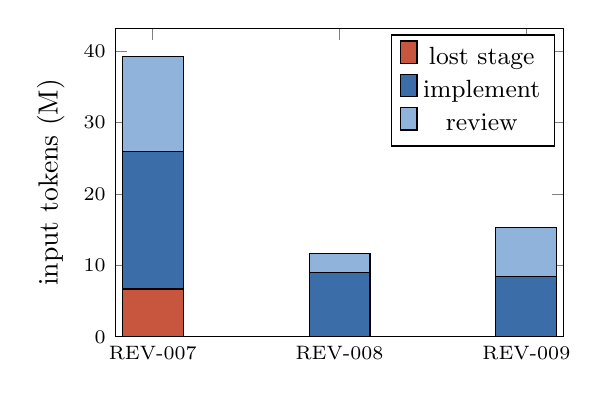
\begin{tikzpicture}
\begin{axis}[ybar stacked, bar width=22pt, width=0.6\linewidth, height=5.5cm,
  symbolic x coords={REV-007,REV-008,REV-009},
  xtick=data, ylabel={input tokens (M)}, ymin=0, legend style={at={(0.98,0.98)},anchor=north east,font=\small},
  tick label style={font=\scriptsize}]
\addplot[fill=waste] coordinates {(REV-007,6.7) (REV-008,0) (REV-009,0)};
\addplot[fill=impl] coordinates {(REV-007,19.3) (REV-008,9.0) (REV-009,8.5)};
\addplot[fill=rev] coordinates {(REV-007,13.3) (REV-008,2.7) (REV-009,6.8)};
\legend{lost stage, implement, review}
\end{axis}
\end{tikzpicture}
\end{center}

Wasted: the first REV-007 stage (6.7M input, \$0.49), whose work was stashed but whose handoff was
unusable. REV-007 took 60\% of the run's input (39.3M of 66.3M) and \$5.73 of \$11.40. Its last
two reopen rounds (\$1.53 review + \$1.22 repair) fixed real but narrow variants of one criterion.

\section*{Comparison with previous runs}

From \texttt{run-log.md}. The previous three-ticket lane, \texttt{qa-layout}: \$5.78 for 3 (\$1.93
each), one reopen, every handoff reaching review on the first attempt. \texttt{ui-screens}: \$13.62
for 3 (\$4.54 each), two reopens. This run: \$11.40 for 3 (\$3.80 each), four reopens, one lost
stage. Two of the three tickets were \texttt{Difficulty: hard} and REV-007 escalated, so 10 of 15
stages ran on Sol xhigh, against none in \texttt{qa-layout}. Reviews cost \$0.60--0.97
(\$0.54--1.08 in \texttt{qa-layout}). REV-008's 25-minute implementation is the lane's longest
stage.

\section*{Observations per model}

\begin{itemize}
  \item \textbf{gpt-6.1-terra xhigh, stage 2} (3 stages, REV-007 only): without the skill it wrote
        a plausible implementation (gate green, 526 tests) but no handoff at all. With the skill it
        worked test-first, with red/green commit pairs. Its tests drove the board through
        \texttt{board.play()} and \texttt{preferences.set\_value()} instead of real input, which is
        how all three round-1 findings slipped. Its repair fixed the reported path but not the
        focused-game entry path.
  \item \textbf{gpt-6.1-sol xhigh, stage 2 (hard)} (5 stages): REV-008 went through on the first
        review, with red/green pairs for each behaviour (handshake, PV2, stop/error, queue). Its
        REV-007 repair for the draw notice special-cases that one node in
        \texttt{\_covers\_settings()} rather than restricting the check to real screens; it
        passed, since the notice was the only offender. On REV-009 it misread criterion 7 (``searches
        nothing new for its class'') as ``no live search on return'' and wrote tests asserting it.
  \item \textbf{gpt-6.1-sol xhigh, review} (7 stages, 4--6~min): every finding came with a real
        viewport or Xvfb reproduction and an external probe on the hard disk. It drip-fed REV-007,
        though: round 1 named only the \texttt{\_covers\_settings} path of criterion 8, and round 2
        missed the draw-notice variant while claiming focused-entry coverage. It authored no fixes;
        it filed CLEAN-014 for long-line scrolling instead of adding it to REV-007.
  \item \textbf{opus-5.5 xhigh, proxy}: one call, granting REV-007's stage 2 the
        \path{ui/main.gd}/\path{ui/review.gd} scope for criteria 1, 2 and 8. All three later
        reviews checked the repairs stayed inside it.
\end{itemize}

\section*{Driver and runtime issues}

\begin{enumerate}
  \item \textbf{Codex had no \texttt{ticket-flow} on the Linux box.} \path{~/.agents/skills} did not
        exist (the earlier P-Chess Codex runs were on Windows), and \path{~/.codex/skills} holds
        only Codex's own skills. EasyMath worked anyway because its \path{AGENTS.md} says a bare-id
        prompt comes from the driver and must load \texttt{ticket-flow}, and Codex then searched
        \path{~/.claude/skills}. P-Chess's \path{AGENTS.md} has no such line. The driver parked the
        bad handoff correctly and stashed the work (\texttt{a3bea32}); its ping checks the proxy
        from each runtime, but not that the runtime can see \texttt{ticket-flow}.
  \item \textbf{New clone needs an import and then a clean.} \texttt{godot --headless --import}
        writes 33 untracked \texttt{.uid}/\texttt{.import} files that \texttt{main} does not track
        yet (the same ones sit untracked in the main checkout); Preflight would refuse the dirty
        tree.
  \item \textbf{Third reopen not parked.} The driver parks only at the second reopen. REV-007's
        third reopen went straight back to stage 2, which was the right call here (the cause was
        already diagnosed), but no rule covers a fourth.
  \item No crash, timeout or API error. Shutdown 0.5--2.3~s per stage. Codex reached the proxy
        directly in all three launches.
\end{enumerate}

\section*{Recommendations}

\begin{enumerate}
  \item Add EasyMath's line to P-Chess's \path{AGENTS.md} (``a bare-id prompt comes from the
        sweatshop driver; load \texttt{ticket-flow} and run the ticket's current stage''), so a
        missing skill install cannot repeat issue 1. The \path{~/.agents/skills} links are in place
        on this box now.
  \item Extend the driver's per-runtime ping to confirm the runtime lists \texttt{ticket-flow} (as
        the foreman's \texttt{codex exec} check did), and stop before the first stage when it does
        not (issue 1).
  \item Commit the 33 generated \texttt{.uid}/\texttt{.import} files to \texttt{main}, so new clones
        and the main checkout stay clean after an import (issue 2).
  \item For UI tickets whose criteria name an interaction (drag, a shortcut, a Settings change),
        write in the ticket's test list that the test drives real viewport input. Every one of
        REV-007's round-1 findings came from tests that called the method behind the input.
  \item Lineup: keep the default Terra lineup with the hard escalation. Scoreboard rows:
        \texttt{gpt-6.1-terra xhigh $\rightarrow$ gpt-6.1-sol xhigh} 101 reviews, 29\% reopened
        (S2 $\geq$28\%), and \texttt{gpt-6.1-sol xhigh $\rightarrow$ gpt-6.1-sol xhigh} 22 reviews,
        23\% (S2 23\%). The Sol pair has more than 10 reviews, but its 22 are mostly hard tickets,
        so the two are not like for like.
\end{enumerate}

\section*{Human debt and proxy decisions}

No \texttt{Débito humano:} lines in this run's tickets. One proxy call, by
\texttt{opus-5.5 xhigh} (Codex reached the proxy directly):

\begin{itemize}
  \item REV-007 (stage 2, after reopen 1): \texttt{Proxy decided (opus-5.5 xhigh)}: ``Yes. Stage 2
        may widen both scopes, limited to the bullets below. Criteria 1, 2 and 8 can't be met
        without these changes, both files are already Primary files, and review R2 sent this
        question to the proxy. Precedent: BOT-005 and CLOCK-001 widened scope the same way.''
        (receipt \path{/tmp/sweatshop-proxy/20261105-175641-REV-007-2bed17.json})
\end{itemize}

\section*{Acceptance}

Checked against the spec's five acceptance scenarios on the integrated session. The code is
identical to REV-009's gated head, so its gate is reused: 554 passed, 0 failed, with the
real-Lc0 checks and one pixel check skipped. The graphical checks come from the stage-3 reviews
under Xvfb, and the record is in \path{.scratch/review-explore/spec.md}, section Acceptance.
\begin{enumerate}
  \item Explore a blunder with real Stockfish: \textbf{pending}, Bruno on Windows. Nothing ran a
        real engine.
  \item Rematch from a side line: \textbf{pass with fakes}
        (\path{tests/test_review.gd}: \texttt{test\_side\_line\_\allowbreak freezes\_queued\_\allowbreak game\_progress\_\allowbreak stop\_works\_\allowbreak and\_rematch\_\allowbreak keeps\_pause}).
  \item Unanalysed or queued game: \textbf{pass with fakes} (the same test and
        \texttt{test\_unanalysed\_side\_line\_\allowbreak settles\_history\_for\_miss\_\allowbreak and\_prunes\_replacements}).
  \item Arrow setting: \textbf{pass}, graphical (Settings over Review, after a focused game, during
        the draw notice).
  \item 800$\times$600: \textbf{pass} on agent captures (\texttt{test\_review\_fits\_an\_\allowbreak 800\_by\_600\_window},
        REV-008's reviewed live capture); Bruno's look pending.
\end{enumerate}
Not examined: real engine output and timing, Threads $=$ cores$-$1 and CPU load, physical promotion
input, and manual play of each exit path.

\section*{Reopen attribution}

Labelled by the foreman (opus-5.5); the reviewer was \texttt{gpt-6.1-sol xhigh}, so no
self-judging. Rows appended to \path{.scratch/reopen-attribution.md}.

{\small\noindent
\begin{tabularx}{\linewidth}{@{}>{\raggedright\arraybackslash}p{1.7cm}X>{\raggedright\arraybackslash}p{2.7cm}X@{}}
\toprule
Ticket (round) & Finding & Label & Why \\
\midrule
REV-007 (1) & Review board ignored real mouse input & S2-explícito/\allowbreak código & criterion 1 names drag and click-click \\
REV-007 (1) & Settings could not open over the Review & S2-explícito/\allowbreak código ? & criterion 8; borderline S1, the repair needed a proxy scope call \\
REV-007 (1) & Played moves lost their animation & S2-explícito/\allowbreak código & criterion 10 names animation length \\
REV-007 (2) & Settings unreachable after a focused game & S2-explícito/\allowbreak código & criterion 8, a supported entry path; review miss and drip-feed \\
REV-007 (3) & Draw notice blocked Settings for 3~s & S2-explícito/\allowbreak código ? & criterion 8; borderline implicit (P3, transient); review miss and drip-feed \\
REV-009 (1) & Stored terminal-draw analysis reused as a before-position & S2-implícito & usable inputs for criteria 2 and 4; the terminal shape is an existing convention \\
REV-009 (1) & Returning to a settled position stopped live analysis & S2-explícito/\allowbreak código ? & criterion 5 and REV-008's live search; borderline S1, criterion 7's wording invited it \\
\bottomrule
\end{tabularx}
}

Totals: S2-explícito/código 6 (3 borderline), S2-implícito 1; no
S1, no S3. Fixed in review: none (the merging reviews authored no behaviour or proof). Review miss
and drip-feed: REV-007 rounds 2 and 3, both on criterion 8. Review-induced churn: none.
No session-review, release-audit or post-release findings yet.

\section*{Scoreboard}

\texttt{scoreboard.ps1} over the ClassyCall, EasyMath, P-Chess, PhysiSyst, SIGAA-ME, SynchroNice and
slip main checkouts (P-Chess with this run's rows, attribution and interventions merged). Moved
since the \texttt{qa-layout} report (EasyMath's lanes ran in between, and \texttt{slip} is new to
the list): implementer \texttt{gpt-6.1-sol xhigh} 10 $\to$ 22 stage runs, still none failed; pair
\texttt{gpt-6.1-sol xhigh} $\rightarrow$ \texttt{gpt-6.1-sol xhigh} 10 $\to$ 22 reviews, 10\%
$\to$ 23\% reopened (this run added 3 of its 5 reopens); pair \texttt{gpt-6.1-terra xhigh}
$\rightarrow$ \texttt{gpt-6.1-sol xhigh} 34 $\to$ 101 reviews, 38\% $\to$ 29\%. Interventions:
automatic-recovery 114 $\to$ 130, proxy-decision (opus-5.5 xhigh) 19 $\to$ 47, human-rescue 32
$\to$ 33.

{\tiny
\begin{verbatim}
| Implementer | Stage runs | To review | Failed | Asked | Median min to review | Cost |
|---|---|---|---|---|---|---|
| gpt-6.1-sol high | 311 | 275 | 12 | 24 | 23m | $839.52 (309/311 priced) |
| opus-5.5 xhigh | 24 | 16 | 8 | 0 | 14m | $100.17 (22/24 priced) |
| gpt-6.1-sol max | 41 | 29 | 9 | 3 | 24m | $84.42 (33/41 priced) |
| opus-5.5 high | 37 | 21 | 15 | 1 | 12m | $73.54 (29/37 priced) |
| gpt-6.1-sol xhigh | 22 | 22 | 0 | 0 | 18m | $57.42 (22/22 priced) |
| gpt-6.1-terra high | 59 | 30 | 27 | 2 | 9m | $9.45 (34/59 priced) |
| gpt-6.1-terra xhigh | 130 | 102 | 18 | 10 | 18m | $107.36 (130/130 priced) |
| gpt-6-astra medium | 57 | 47 | 1 | 9 | 10m | $162.72 (57/57 priced) |
(other implementer rows omitted: unchanged models outside this lineup)

| Implementer | Reviewer | Reviews | Reopened | Reopen rate | Reopened for S2 | S2 rate | Unclassified | Fixed in review for S2 |
|---|---|---|---|---|---|---|---|---|
| gpt-6.1-sol high | gpt-6.1-sol xhigh | 176 | 33 | 19% | 32 | 18% | 0 | 20 |
| gpt-6.1-sol max | gpt-6.1-sol xhigh | 9 | 2 | 22% | 2 | 22% | 0 | 0 |
| gpt-6.1-sol xhigh | gpt-6.1-sol xhigh | 22 | 5 | 23% | 5 | 23% | 0 | 1 |
| opus-5.5 high | gpt-6.1-sol xhigh | 1 | 1 | 100% | 1 | 100% | 0 | 0 |
| gpt-6.1-terra high | gpt-6.1-sol xhigh | 30 | 7 | 23% | 7 | 23% | 0 | 0 |
| ? | gpt-6.1-sol xhigh | 7 | 2 | 29% | 1 | 14% | 0 | 0 |
| gpt-6.1-terra xhigh | gpt-6.1-sol xhigh | 101 | 29 | 29% | 28 | >=28% | 1 | 12 |
(pairs under other reviewers omitted)

| Implementer -> Reviewer | Rounds | S2 explicit code | S2 explicit test | S2 implicit | S1 | S3 noise |
|---|---|---|---|---|---|---|
| gpt-6.1-sol xhigh -> gpt-6.1-sol xhigh | 5 | 6 | 0 | 2 | 0 | 0 |
| gpt-6.1-terra high -> gpt-6.1-sol xhigh | 9 | 10 | 1 | 3 | 1 | 0 |
| gpt-6.1-terra xhigh -> gpt-6.1-sol xhigh | 40 | 50 | 2 | 12 | 4 | 0 |

| Discovery | Recorded findings | Earlier review miss (yes / known) | Review-induced churn (yes / known) |
|---|---|---|---|
| release-audit | 2 | 2 / 2 | 0 / 2 |
| session-review | 36 | 29 / 31 | 0 / 31 |
| ticket-review | 395 | 9 / 256 | 1 / 258 |
Runtime completion to process exit: 1618.016s total over 1196 measured stages; 773 unmeasured.
| Intervention | Recorded events |
|---|---|
| automatic-recovery | 130 |
| human-rescue | 33 |
| proxy-decision (gpt-6-astra high, fallback) | 58 |
| proxy-decision (opus-5.5 xhigh) | 47 |
| proxy-decision (opus) | 42 |
| proxy-decision (supervisor) | 12 |
| proxy-decision (unknown) | 37 |
| routine-approval | 18 |
\end{verbatim}
}

Under the same reviewer, Terra xhigh (101 reviews) reopens more than Sol xhigh (22) and Terra
high (30). The Sol xhigh pair only sees hard or escalated tickets, so it is not a like-for-like
comparison.

\section*{Pending for the human}

\begin{enumerate}
  \item On Windows with real Stockfish, before merging PR \#42 (REV-008 and REV-009 are
        \texttt{Review: human}): open an analysed game from History at a Blunder, drag another
        move, watch depth rise and the icon arrive; click moves in an engine line; Back to game;
        Rematch from a side line; explore a queued game and watch the queue pause and resume. Watch
        CPU load.
  \item By hand, post-game and from History: start a side line, overwrite it, walk it, leave it
        each way; toggle Best move arrow in Settings while the Review is open, including after an
        F11 game.
  \item Decide on adding the ``bare id loads \texttt{ticket-flow}'' line to P-Chess's
        \path{AGENTS.md} (recommendation 1).
  \item Triage CLEAN-014 (long side lines do not scroll to the current row).
  \item After merging PR \#42, tell the other open lanes' foremen to sync.
\end{enumerate}

\end{document}
